% \chapter{Simulação e Resultados}
\chapter{Experimentos}

Para este trabalho foram realizados três experimentos com o objetivo de averiguar se o modelo HAIL é funcional ou não. Esses experimentos não possuem um domínio específico, ou seja, não há um ambiente real onde o agente está inserido, ele recebe percepções aleatórias geradas pelo simulador e os planos inicias do agente não são relevantes para os testes.

Os dois primeiros experimentos foram implementados utilizando o design $2^k$ fatorial \cite{jain1990art}. Esse tipo de design consiste em variar $k$ fatores em 2 níveis diferentes, -1 e 1, que são extremos opostos. Por exemplo, em uma pesquisa ligada a um processador, um fator pode ser o número de núcleos, e seus níveis serem 1 núcleo e 8 núcleos. O fator é uma variável livre, utilizada para analisar a variação de uma variável dependente qualquer. Os fatores e as variáveis livres utilizadas estão nas Tabelas \ref{table:experiments_factors} e \ref{table:experiments_variables}, respectivamente. A análise do impacto dos fatores foi realizada utilizando a equação de regressão não linear do design $2^k$ fatorial.
%O código implementado para essa análise está disponível no anexo [NÚMERO].

\begin{table}[h!]
    \begin{center}
        \caption{ Fatores utilizados nos experimentos realizados com o modelo HAIL. }
        \label{table:experiments_factors}
        \begin{tabular}{|c|c|c|c|}
        \hline
        \textbf{Fatores} & \textbf{Sigla} & \textbf{Nível -1} & \textbf{Nível 1} \\
        \hline
        Porcentagem de Percepções Inválidas & PPI & 5\% & 95\%  \\
        \hline
        Tempo Médio gasto pelo planejamento Automatizado & TMA & 1/2 T & 64 T \\
        \hline
        Tempo Médio gasto em um Ciclo de raciocínio & TMC & 01 T & 32 T \\
        \hline
        Número de Percepções recebidas por Ciclo & NPC & 01 & 16 \\
        \hline
    \end{tabular}{}
    \legend{Fonte: Autor.}
    \end{center}
\end{table}{}

\begin{table}[h!]
    \begin{center}
        \caption{ Variáveis dependentes analisadas nos experimentos realizados com o modelo HAIL. }
        \label{table:experiments_variables}
        \begin{tabularx}{\textwidth}{ |Y|Y| }
            \hline
            \textbf{Variáveis} & \textbf{Motivação} \\
            \hline
            Tempo Virtual Decorrido & Medir desempenho geral do modelo \\
            \hline
            Planos Criados & Avaliar potencial do modelo de inserir aprendizado em arquiteturas que não o possuem \\
            \hline
            Percepções Válidas Processadas & Analisar a capacidade do modelo de ganhar desempenho ao longo do tempo\\
            \hline
        \end{tabularx}{}
    \legend{Fonte: Autor.}
    \end{center}{}
\end{table}

O terceiro experimento não utiliza o design $2^k$ fatorial. Após as simulações do segundo experimento, foi identificada a demanda de analisar como o HAIL era impactado com o processo contínuo de aprendizado fornecido pelo bloco de planejamento automatizado. Este experimento não utiliza um design específico, e será melhor explicado na Seção \ref{section:exp3}.

Os experimentos consistem em diversas simulações, que submetem o modelo proposto ao processo de revisão de um grande número de percepções. Uma simulação possui 5000 ciclos de percepção, sendo que cada ciclo pode possuir uma ou várias percepções. Essas percepções podem ser válidas (pertencentes ao contexto do agente) ou inválidas (não pertencentes ao contexto do agente), sendo que a proporção entre o tipo de percepções é definido pela PPI. As percepções são produzidas aleatoriamente por um gerador de percepções. 

O gerador de percepções cria as percepções válidas sorteando símbolos que pertencem ao contexto do agente, e as percepções inválidas são criadas utilizando o pacote \texttt{RandomWords} \cite{pipRandomWords2}, que gera palavras em inglês aleatórias. As percepções são símbolos compostos da forma \texttt{corpo(argumento)}, e a quantidade de percepções válidas e inválidas geradas é baseado no PPI e TMA da simulação executada.

Cada ciclo da simulação segue os seguintes passos:

\begin{enumerate}
    \item Gerar as percepções da simulação;
    \item Iterar sobre cada um dos ciclos, passando as percepções para o modelo implementado;
    \item Salvar os resultados, o agente final (com novos planos gerados pelo módulo de planejamento automatizado) e as percepções de cada ciclo em arquivos CSV.
\end{enumerate}

\begin{figure}[h!]
    \centering
    \caption{Diagrama da execução de uma iteração de cada simulação.}
    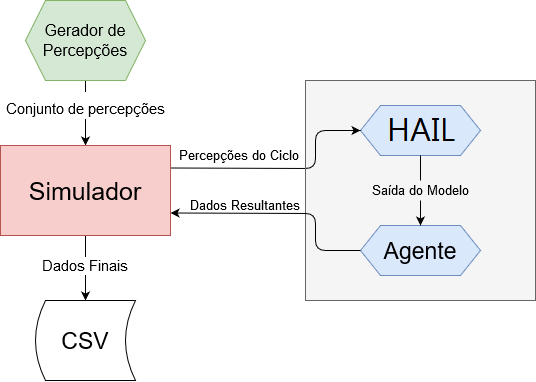
\includegraphics[width=0.8\textwidth]{images/diagrama-simulacao.png}
    \legend{Fonte: Autor.}
    \label{fig:diagrama-simulacao}
\end{figure}

Além da configuração dos valores dos fatores, é possível configurar se um agente será recarregado (ou seja, se ele deve manter os planos gerados por uma simulação anterior) e se o simulador deve gerar novas percepções ou não, pulando a etapa 1 de cada ciclo.

Para mensurar o tempo gasto pelos processos do agente, será considerada uma unidade de tempo genérica T, e iremos considerar o tempo virtual da execução das simulações com base nessa unidade. Portanto em uma simulação que possui TMC de 1T e TMA de 64T, o tempo médio do planejamento automatizado é 64 vezes maior do que o tempo médio do ciclo de raciocínio do agente.

Foi utilizado o agente do Exemplo \ref{example::robo} nas simulações, mas ele não foi descrito de acordo com nenhuma linguagem de programação de agentes real. Suas regras utilizam o formato de notação $percepcao -> acao1; acao2; ...; acaoN$. As ações desta implementação, assim como as percepções, são símbolos da forma \texttt{corpo(argumento)}. O módulo de refinamento não foi implementado, ou seja, sua entrada e saída são equivalentes.

\section{Implementação}

A implementação do simulador foi feita em Python 3.7, e conta com três classes principais: \texttt{PerceptionGenerator}, \texttt{PerceptionRevision} e \texttt{Simulator}. As interações das classes do simulador a partir do método \texttt{main} estão ilustradas na Figura \ref{fig:diagrama-implementacao}.

\begin{figure}
    \centering
    \caption{Diagrama demonstrando o relacionamento entre as classes do simulador.}
    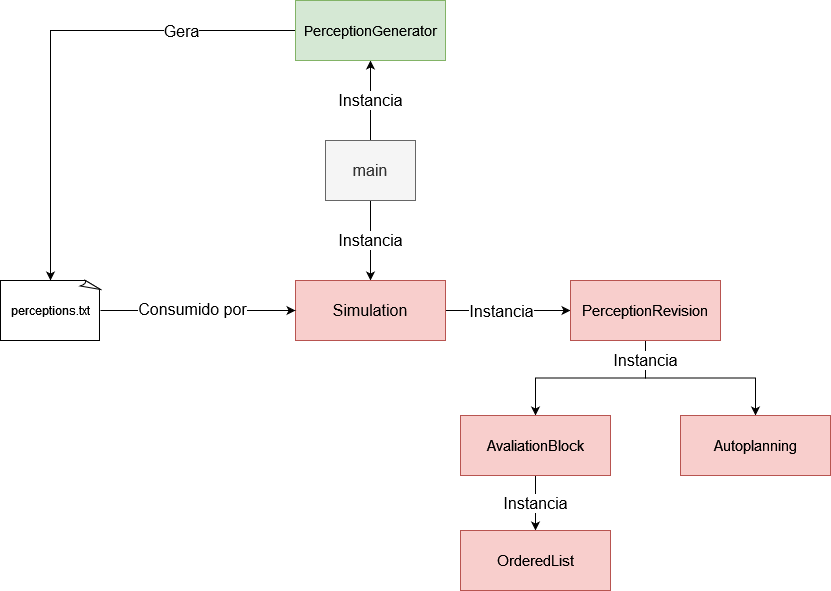
\includegraphics[width=\textwidth]{images/diagrama-implementacao.png}
    \legend{Fonte: Autor.}
    \label{fig:diagrama-implementacao}
\end{figure}

O gerador de percepções foi abstraído em um pacote chamado de \texttt{generator}, e sua classe é implementada no arquivo \texttt{perceptions.py}. Esta classe deve ser instanciada passando como argumento o número de ciclos de percepção que serão utilizados na simulação, a porcentagem de percepções inválidas e o número de percepções por ciclo. Depois de instanciado, é possível utilizar o objeto para chamar a função \texttt{generate}, que utiliza a configuração recebida para criar as percepções e escrevê-las num arquivo \texttt{perceptions.txt}. As percepções inválidas são geradas aleatoriamente com o pacote \texttt{RandomWords} e as percepções válidas são geradas a partir da especificação do arquivo \texttt{perceptions\_options.py}, onde são definidas o corpo e o argumento das percepções válidas.

O modelo HAIL foi implementado na classe \texttt{PerceptionRevision}, que está contido no arquivo \texttt{pr\_system.py}. Ele implementa cada um dos processos descritos no Capítulo \ref{chapter:model}. Quando esta classe é instanciada, ela primeiro extrai o contexto do agente através do método auxiliar \texttt{get\_agent\_context}, que percorre o arquivo do agente buscando os símbolos que compõem o contexto no corpo e no argumento dos símbolos dos planos. Depois disso, são instanciados os blocos de avaliação como atributos da classe do revisor, um para cada tipo de anomalia. Eles são implementados em uma classe chamada \texttt{AvaliationBlock}. Cada bloco guarda uma instância da classe \texttt{OrderedList}, que representa a lista ordenada definida pelo modelo. Por último, o bloco de planejamento \texttt{Autoplanner} é instanciado.

Como o bloco de planejamento automatizado não é o foco do trabalho, e possui uma grande complexidade de implementação, foi criado uma versão que cria um plano novo juntando a anomalia recebida com um conjunto aleatório de ações que o agente possui. Além disso, nessa implementação alucinações e ilusões utilizam o mesmo método de planejamento automatizado, portanto apenas um bloco é instanciado.

A anomalia \texttt{studies(distortion)} submetida ao planejamento automatizado pode gerar a percepção \texttt{studies(distortion) -> wrap\_up(circle)}, por exemplo. A implementação do \texttt{Autoplanner} gera um número aleatório de ações por plano, podendo ser uma ou no máximo o número de ações que o agente possui (nesse caso dois). 

O revisor de percepções possui um método principal utilizado nas simulações chamado \texttt{process\_perceptions}, que recebe uma lista de percepções, submete cada percepção ao fluxo do HAIL e então retorna o tempo virtual decorrido e o número de percepções válidas processadas. Para isso, cada percepção é classificada pelos decisores do módulo de alucinação e ilusão e então adicionada ao bloco avaliador designado. Quando todas as percepções foram classificadas, o modelo escolhe se vai processar as ilusões ou alucinações primeiro. Nessa implementação, essa escolha é feita aleatoriamente. Os blocos avaliadores passam pelo processo de validação da função de processamento, e anomalias são enviadas para o planejamento automatizado enquanto a função retornar verdadeiro.

Por fim, a classe \texttt{Simulation} utiliza as duas classes descritas anteriormente para executar a simulação. As percepções do arquivo \texttt{perceptions.txt} são lidas pelo método \texttt{run}, executando cada um dos ciclos de percepção utilizando uma instância da classe \texttt{PerceptionRevision}. Os valores finais de tempo virtual, percepções processadas e planos criados são retornados e guardados em um arquivo CSV.

Além da simulação, outro projeto foi criado para analisar o impacto dos fatores, medir o erro dos experimentos e criar os gráficos. Ele também foi implementado em Python 3.7 e utiliza as ferramentas \texttt{pandas} \cite{reback2020pandas}, \texttt{matplotlib} \cite{Hunter:2007} e \texttt{seaborn} \cite{Waskom_seaborn_statistical_data_2021}.

\section{Experimento 1}

O objetivo do primeiro experimento é analisar o impacto da mudança dos fatores no desempenho do modelo através da analise da variação no tempo virtual decorrido e da quantidade de planos criados pelo módulo de planejamento automatizado. 

Esse experimento foi o primeiro realizado com a metodologia do  $2^k$ fatorial. Cada um dos fatores foi avaliado em ambos os níveis apresentados na Tabela \ref{table:experiments_factors}, resultando em dezesseis combinações diferentes, e portanto dezesseis simulações. O tempo virtual foi escolhido para termos uma métrica geral de desempenho do sistema, enquanto a quantidade de planos criadas foi escolhida por ser um dos principais diferenciais do sistema, e um de seus aspectos mais importantes.

Cada simulação foi repetida dez vezes, e a média dos resultados foi obtida. Isso foi feito para garantir que os valores obtidos não foram afetados pela geração aleatória de percepções. Quando repetições são adotadas no experimento normalmente utiliza-se a metodologia $2^k r$ fatorial, que leva em conta o erro obtido entre as diferentes execuções da simulação. Todavia, ao fazer a análise de erros o resíduo obtido foi descartável, com ordem de grandeza $e^{-12}$. Portanto, a metodologia de análise adotada foi a do  $2^k$ fatorial.

\subsection{Resultados}

As médias dos resultados de cada simulação estão apresentadas na Tabela \ref{table:experimento1}. O valor final do tempo virtual decorrido varia bastante, principalmente nas simulações com alto nível de percepções inválidas. Em dois momentos o tempo virtual foi 5000T. Esse valor exato se repetiu pois nessas simulações o TMC é 1, o TMA é 0.5 e o NPC é 16. Nessa configuração os ciclos de percepções válidas consumiam 1 unidade de tempo, totalizando um tempo virtual de 4750T. O bloco avaliado sempre permitia o processamento de 2 percepções inválidas (pois cada uma toma 0.5 unidades de tempo), e quase sempre há percepções inválidas disponíveis na fila pois entram 16 percepções inválidas por ciclo de percepções inválidas. Portanto, cada vez que o modelo processava percepções inválidas, ele consumia 1 unidade de tempo, e isso aconteceu 250 vezes (5\% de 5000).

\begin{table}[h!]
    \begin{center}
        \caption{ Resultados do experimento 1.}
        \label{table:experimento1}
        \begin{tabular}{ |c|c|c|c|c|c|c| }
            \hline
            \textbf{Simulação} & \textbf{PPI} & \textbf{TMC} & \textbf{TMA} & \textbf{NPC} & \textbf{Tempo Virtual} & \textbf{Planos Criados}\\
            \hline
            1 & 5\% & 1 & 1/2 & 1 & 4874.6T & 250.8\\
            \hline
            2 & 5\% & 1 & 1/2 & 16 & 5000.0T & 502.0\\
            \hline
            3 & 5\% & 1 & 64 & 1 & 20806.7T & 250.9\\
            \hline
            4 & 5\% & 1 & 64 & 16 & 20813.0T & 251.0\\
            \hline
            5 & 5\% & 32 & 1/2 & 1 & 152093.5T & 251.0\\
            \hline
            6 & 5\% & 32 & 1/2 & 16 & 153437.3T & 2932.2\\
            \hline
            7 & 5\% & 32 & 64 & 1 & 168028.8T & 250.9\\
            \hline
            8 & 5\% & 32 & 64 & 16 & 168032.0T & 251.0\\
            \hline
            9 & 95\% & 1 & 1/2 & 1 & 3229.2T & 3541.6\\
            \hline
            10 & 95\% & 1 & 1/2 & 16 & 5000.00T & 9303.8\\
            \hline
            11 & 95\% & 1 & 64 & 1 & 228668.9T & 3550.3\\
            \hline
            12 & 95\% & 1 & 64 & 16 & 304300.4T & 4750.8\\
            \hline
            13 & 95\% & 32 & 1/2 & 1 & 48521.5T & 3539.0\\
            \hline
            14 & 95\% & 32 & 1/2 & 16 & 140683.3T & 4073.8\\
            \hline
            15 & 95\% & 32 & 64 & 1 & 273609.6T & 3550.3\\
            \hline
            16 & 95\% & 32 & 64 & 16 & 312032.0T & 4751.0\\
            \hline
        \end{tabular}{}
    \legend{Fonte: Autor.}
    \end{center}{}
\end{table}

O número de planos criados se agruparam em certos conjuntos de valores, de acordo com os níveis dos fatores. Como esperado, as simulações com menor porcentagem de percepções inválidas criaram menos planos, pois houveram menos anomalias, logo menos material para o módulo de planejamento automatizado trabalhar. A Figura \ref{fig:pc_occurrences} mostra a ocorrência de valores próximos de planos criados para cada uma das faixas obtidas nas simulações. Por exemplo, as simulações 12 e 16 tiveram aproximadamente 4750 percepções criadas, portanto foram agrupadas na mesma faixa no gráfico. Essas faixas de valores indicam que há uma discrepância entre as simulações com PPI de 5\% (com 6 ocorrências de aproximadamente 250 planos criados) e as simulações com PPI 95\%. Com isso, é possível notar que a principal condição para que o bloco de planejamento automatizado crie uma quantidade elevada de planos novos é um grande percentual de anomalias em relação ao total de percepções recebidas.

\begin{figure}[h!]
    \centering
    \caption{Recorrência do valor final de Planos Criados nas simulações realizadas.}
    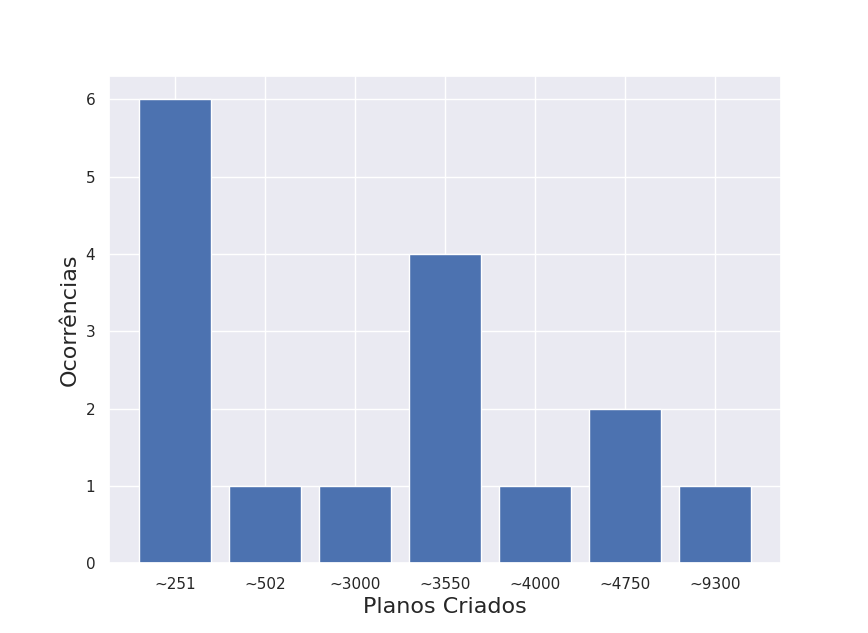
\includegraphics[width=1\textwidth]{images/plans_created_occurrences.png}
    \legend{Fonte: Autor.}
    \label{fig:pc_occurrences}
\end{figure}

\subsection{Análise de fatores}

Conforme mostra a Tabela \ref{tab:experimento1fatores}, na variável dependente de Tempo Virtual, os fatores TMC e TMA isolados tiveram uma alta porcentagem de impacto. Isso porque a contagem do tempo virtual acontece em função do tempo médio do ciclo de raciocínio e do tempo médio do planejamento automatizado. Portanto, a interferência nesses fatores influencia diretamente o resultado final. Além disso, a combinação dos fatores PPI + TMA teve um impacto de 24.13\%. Isoladamente, PPI e TMA possuem porcentagens altas (12.69 e 31.64, respectivamente) e quanto mais percepções inválidas há, maior o tempo gasto no planejamento automatizado, pois mais anomalias podem ser processadas. Como cada fator possui impacto alto e seus valores interferem diretamente um com o outro, a combinação de ambos acaba sendo relevante para o resultado das simulações. Por outro lado, TMC possui 22.20\% de impacto, mas a combinação PPI + TMC possui apenas 4.16, pois a porcentagem de percepções inválidas não interage diretamente com o tempo gasto no ciclo de raciocínio.

Isso demonstra como uma combinação de alta taxa de percepções inválidas com um tempo de planejamento automatizado alto podem ser impactantes no NPC. Portanto, em situações com um grande volume de percepções, implementações que possuem um bloco de planejamento automatizado que consome muito tempo para criar novos planos podem prejudicar o desempenho do agente caso ele seja muito sensível ao tempo.

\begin{table}
    \begin{center}
        \caption{Análise dos fatores do experimento 1.}
        \label{tab:experimento1fatores}
        \begin{tabular}{ |c|c|c| }
            \hline
            \textbf{Fator} & \textbf{Efeito Tempo Virtual} & \textbf{Efeito Planos Criados}\\  
            \hline
            PPI & 12.69\% & 66.10\%\\
            \hline
            TMC & 22.20\% & 0.50\%\\
            \hline
            TMA & 31.64\% & 2.95\%\\
            \hline
            NPC & 1.44\% & 8.67\%\\
            \hline
            PPI + TMC & 4.16\% & 3.76\%\\
            \hline
            PPI + TMA & 24.13\% & 0.05\%\\
            \hline
            PPI + NPC & 1.39\% & 2.13\%\\
            \hline
            TMC + TMA & 0.55\% & 0.50\%\\
            \hline
            TMC + NPC & 0.10\% & 0.50\%\\
            \hline
            TMA + NPC & 0.01\% & 2.99\%\\
            \hline
            PPI + TMC + TMA & 0.53\% & 3.76\%\\
            \hline
            PPI + TMC + NPC & 0.09\% & 3.75\%\\
            \hline
            PPI + TMA + NPC & 0.02\% & 0.06\%\\
            \hline
            TMC + TMA + NPC & 0.54\% & 0.50\%\\
            \hline
            PPI + TMC + TMA + NPC & 0.52\% & 3.76\%\\
            \hline
        \end{tabular}{}
    \legend{Fonte: Autor.}
    \end{center}{}
\end{table}


Na variável dependente Planos Criados, o fator que mais impactou o resultado foi o PPI. Isso era o esperado, pois quanto mais percepções inválidas o modelo recebe, mais planos podem ser criados. Os demais fatores tiveram impactos mais baixos. O NPC teve 8.67\% de influência pois simulações com mais percepções inválidas por ciclo preenchem a fila ponderada mais rápido, permitindo que o bloco avaliador sempre possua elementos na fila ponderada para enviar ao bloco de planejamento automatizado.

%%%%%%%%%%%%%%%%%%%%%%%%%%%%%%%%%%%%%%%%%%%%%%%%%%%%%%%%%%%%%%%%%%%%

\section{Experimento 2}

O segundo experimento foi realizado para analisar o ganho de performance de um agente ao utilizar os planos criados com o bloco de planejamento automatizado. Esse segundo experimento segue a metodologia do primeiro, porém foi realizado apenas uma iteração para cada configuração de fatores (ao invés das dez repetições). Após ser realizada uma simulação com uma configuração de fatores foi realizada uma nova simulação com a mesma configuração, mas usando o agente resultante da primeira. Assim, os planos criados pelo agente foram reaproveitados. Ao invés de analisar quais são os fatores que mais influenciam nas variáveis dependentes, comparamos os resultados dessas variáveis antes e depois da criação de novos planos. As variáveis dependentes analisadas foram novamente o tempo virtual decorrido e o número de planos criados.

% Como a segunda simulação sempre vai ter menos planos criados que a primeira (pois o agente já passou pelo processo de aprendizado), as variáveis dependentes analisadas foram o tempo virtual decorrido e o número de planos criados. Essa nova variável foi escolhida pois caso o TMC for alto, na segunda simulação o tempo virtual será maior, pois o agente aprendeu novos planos e portanto menos percepções serão anomalias. Todavia, o tempo virtual não é capaz de mensurar o aprendizado do agente. Como um dos principais objetivos do HAIL é fornecer aprendizado, a métrica de percepções processadas ajuda a medir a redução de anomalias na segunda simulação.

Esse experimento pode ter sua configuração de fatores separadas em dois grupos: (I) o tempo de processamento de um ciclo de raciocínio é menor do que o tempo do planejamento automatizado; (II) o tempo do planejamento automatizado é menor que o tempo de processamento de um ciclo de raciocínio. Essa separação pode ser feita pois quanto mais planos são criados, menos percepções inválidas serão recebidas pelo agente. Portanto, se o tempo de processamento de um ciclo for maior que o da geração de novos planos, o tempo virtual gasto total usando um agente que já aprendeu vários planos será maior. Isso é uma troca realizada pois agora essas novas percepções (que eram antes anomalias) estão sendo recebidas pelo agente e resultando na execução de um plano.

\subsection{Resultados}

Os resultados estão separados em tabelas por variável dependente e por grupo, como descrito anteriormente. As tabelas contém o índice da simulação, os níveis dos fatores, os resultados da primeira e da segunda iteração (R1 e R2, respectivamente) e a relação percentual (RP) entre os resultados, ou seja, a proporção de R2 em relação a R1, obtido através do cálculo $(R2 * 100) / R1$.

Em todas as tabelas, podem ser observadas um menor efeito na relação percentual nas simulações que utilizaram o nível $-1$ do fator PPI (5\% de percepções inválidas). Isso acontece pois o modelo possui menor impacto em ambientes de baixo volume de percepções inválidas, uma vez que o bloco de planejamento automatizado apenas cria novos planos quando há percepções inválidas na fila ponderada do bloco avaliador.

Na Tabela \ref{table:vtaltv1}, a média da relação percentual foi de 75.26\%, se destacando a simulação 5 com uma relação percentual de 4.77\%. Com o tempo de planejamento automatizado alto, tempo de processamento de um ciclo de raciocínio baixo e apenas uma percepção por ciclo, há um grande ganho de desempenho, conforme explicado anteriormente. Um comportamento similar (porém invertido) pode ser observado na Tabela \ref{table:vtaltv2}, cuja média da relação percentual foi de 136.33\%. Nessas simulações, o esperado era que o tempo virtual subisse conforme a quantidade de planos criados aumentasse, pois o tempo gasto no planejamento automatizado é menor que o tempo gasto no ciclo de raciocínio.

\begin{table}
    \begin{center}
        \caption{Alteração no valor de tempo virtual nas simulações do grupo I.}
        \label{table:vtaltv1}
        \begin{tabular}{ |c|c|c|c|c|c|c|c| }
            \hline
            \textbf{Simulação} & \textbf{PPI} & \textbf{TMC} & \textbf{TMA} & \textbf{NPC} & \textbf{R1} & \textbf{R2} & \textbf{RP}\\
            \hline
            1.1 & 5\% & 1 & 64 & 1 & 20750T & 20687T & 99.70\%\\
            \hline
            1.2 & 5\% & 1 & 64 & 16 & 20813T & 20750T & 99.70\%\\
            \hline
            1.3 & 5\% & 32 & 64 & 1 & 168032T & 167968T & 99.96\%\\
            \hline
            1.4 & 5\% & 32 & 64 & 16 & 168032T & 168000T & 99.98\%\\
            \hline
            1.5 & 95\% & 1 & 64 & 1 & 227579T & 10859T & 4.77\%\\
            \hline
            1.6 & 95\% & 1 & 64 & 16 & 304313T & 177998T & 58.49\%\\
            \hline
            1.7 & 95\% & 32 & 64 & 1 & 273536T & 162400T & 59.37\%\\
            \hline
            1.8 & 95\% & 32 & 64 & 16 & 312032T & 250048T & 80.14\%\\
            \hline
            
        \end{tabular}{}
    \legend{Fonte: Autor.}
    \end{center}{}
\end{table}

\begin{table}
    \begin{center}
        \caption{ Alteração no valor de tempo virtual nas simulações do grupo II. }
        \label{table:vtaltv2}
        \begin{tabular}{ |c|c|c|c|c|c|c|c| }
            \hline
            \textbf{Simulação} & \textbf{PPI} & \textbf{TMC} & \textbf{TMA} & \textbf{NPC} & \textbf{R1} & \textbf{R2} & \textbf{RP}\\
            \hline
            2.1 & 5\% & 1 & 1/2 & 1 & 4874.5T & 4876.5T & 100.04\%\\
            \hline
            2.2 & 5\% & 1 & 1/2 & 16 & 5000T & 5000T & 100\%\\
            \hline
            2.3 & 5\% & 32 & 1/2 & 1 & 152093.5T & 152219.5T & 100.08\%\\
            \hline
            2.4 & 5\% & 32 & 1/2 & 16 & 153435.5T & 152887T & 99.64\%\\
            \hline
            2.5 & 95\% & 1 & 1/2 & 1 & 3228.5T & 4955T & 153.48\%\\
            \hline
            2.6 & 95\% & 1 & 1/2 & 16 & 5000T & 4944T & 98.88\%\\
            \hline
            2.7 & 95\% & 32 & 1/2 & 1 & 48458.5T & 157385.5T & 324.78\%\\
            \hline
            2.8 & 95\% & 32 & 1/2 & 16 & 160000T & 140631T & 113.77\%\\
            \hline
            
        \end{tabular}{}
    \legend{Fonte: Autor.}
    \end{center}{}
\end{table}

A outra variável analisada foi o número de percepções válidas processadas. A média de cada configuração de fatores foi de 30563.0625 percepções, enquanto nas segundas simulações foi de 40599.75, totalizando um ganho aproximado de 32.84\% de desempenho. Ou seja, apesar do ganho de tempo virtual em algumas situações, um maior número de percepções foi processada e resultou na execução de um plano do agente.

As Tabelas \ref{table:plansaltv1} e \ref{table:plansaltv2} mostram a variação do ganho de planos criados entre as simulações. Ambas apresentam uma queda drástica nessa variável nas simulações com 95\% de percepções inválidas, pois foram nessas simulações que o modelo pode criar mais planos (pois o planejamento automatizado é utilizado mais vezes). As simulações 1.6 e 1.8 possuem um resultado acima das
simulações 1.5 e 1.7, apesar das quatro possuírem PPI de 95\%, pois possuem mais percepções (16 vezes mais por conta do NPC) e processam no máximo uma percepção inválida por ciclo (pois o TMA é maior que o TMC).
A Tabela \ref{table:plansaltv2} possui valores ainda menores na relação percentual pois muitas percepções inválidas são processadas por ciclo, em especial na simulação 2.8, onde nenhum plano novo foi criado na segunda simulação. Isso ocorreu pois o TMC é alto, o TMA é baixo e ela possui o maior número possível de percepções inválidas, resultando em um uso constante do planejamento automatizado.

\begin{table}
    \begin{center}
        \caption{ Alteração no valor de planos criados nas simulações do grupo I. }
        \label{table:plansaltv1}
        \begin{tabular}{ |c|c|c|c|c|c|c|c| }
            \hline
            \textbf{Simulação} & \textbf{PPI} & \textbf{TMC} & \textbf{TMA} & \textbf{NPC} & \textbf{R1} & \textbf{R2} & \textbf{RP}\\
            \hline
            1.1 & 5\% & 1 & 64 & 1 & 250.0 & 249.0 & 99.60\%\\
            \hline
            1.2 & 5\% & 1 & 64 & 16 & 251.0 & 250.0 & 99.60\%\\
            \hline
            1.3 & 5\% & 32 & 64 & 1 & 251.0 & 249.0 & 99.20\%\\
            \hline
            1.4 & 5\% & 32 & 64 & 16 & 251.0 & 250.0 & 99.60\%\\
            \hline
            1.5 & 95\% & 1 & 64 & 1 & 3533.0 & 93.0 & 2.63\%\\
            \hline
            1.6 & 95\% & 1 & 64 & 16 & 4751.0 & 2746.0 & 57.80\%\\
            \hline
            1.7 & 95\% & 32 & 64 & 1 & 3548.0 & 75.0 & 2.11\%\\
            \hline
            1.8 & 95\% & 32 & 64 & 16 & 4751.0 & 2814.0 & 59.23\%\\
            \hline
            
        \end{tabular}{}
    \legend{Fonte: Autor.}
    \end{center}{}
\end{table}


\begin{table}
    \begin{center}
        \caption{ Alteração no valor de planos criados nas simulações do grupo II. }
        \label{table:plansaltv2}
        \begin{tabular}{ |c|c|c|c|c|c|c|c| }
            \hline
            \textbf{Simulação} & \textbf{PPI} & \textbf{TMC} & \textbf{TMA} & \textbf{NPC} & \textbf{R1} & \textbf{R2} & \textbf{RP}\\
            \hline
            2.1 & 5\% & 1 & 1/2 & 1 & 251.0 & 247.0 & 98.41\%\\
            \hline
            2.2 & 5\% & 1 & 1/2 & 16 & 502.0 & 500.0 & 99.60\%\\
            \hline
            2.3 & 5\% & 32 & 1/2 & 1 & 251.0 & 247.0 & 98.41\%\\
            \hline
            2.4 & 5\% & 32 & 1/2 & 16 & 2935.0 & 878.0 & 29.91\%\\
            \hline
            2.5 & 95\% & 1 & 1/2 & 1 & 3543.0 & 90.0 & 2.54\%\\
            \hline
            2.6 & 95\% & 1 & 1/2 & 16 & 9312.0 & 260.0 & 2.79\%\\
            \hline
            2.7 & 95\% & 32 & 1/2 & 1 & 3541.0 & 83.0 & 2.34\%\\
            \hline
            2.8 & 95\% & 32 & 1/2 & 16 & 4078.0 & 0.0 & 0.0\%\\
            \hline
            
        \end{tabular}{}
    \legend{Fonte: Autor.}
    \end{center}{}
\end{table}

\section{Experimento 3}

\label{section:exp3}

O terceiro experimento foi executado para observar a capacidade de aprendizado do agente ao longo do tempo. Nele foram executadas 5 simulações com os mesmos fatores dos experimentos anteriores, mas com valores diferentes (como demonstra a Tabela \ref{table:experiment3factors}). Entre uma simulação e outra o agente não foi recarregado, ou seja, manteve o aprendizado das simulações anteriores.

\begin{table}[h!]
    \begin{center}
        \caption{ Valor dos fatores no experimento 3. }
        \label{table:experiment3factors}
        \begin{tabular}{ |c|c| }
            \hline
            \textbf{Fator} & \textbf{Valor}\\
            \hline
            PPI & 50\%\\
            \hline
            TMC & 16\\
            \hline
            TMA & 32\\
            \hline
            NPC & 8\\
            \hline
        \end{tabular}{}
    \legend{Fonte: Autor.}
    \end{center}{}
\end{table}

Os resultados estão expostos na Tabela \ref{table:experiment3results}, mostrando o comportamento dos três fatores observados. Enquanto os planos criados diminuem a cada simulação, pois menos percepções são inválidas (uma vez que o agente aprende com as simulações anteriores), a quantidade de percepções válidas processadas aumenta. Esse comportamento é demonstrado na Figura \ref{fig:perceptions_v_plans-experiment3}. Além disso, o tempo virtual cai na mesma proporção que os planos criados diminuem, uma vez que a criação de um plano é duas vezes mais custosa em tempo do que o processamento de uma percepção válida nesse experimento.

\begin{table}
    \begin{center}
        \caption{ Resultados obtidos no experimento 3. }
        \label{table:experiment3results}
        \begin{tabular}{ |c|c|c|c| }
            \hline
            \textbf{Simulação} & \textbf{Planos Criados} & \textbf{Percepções Válidas Processadas} & \textbf{Tempo Virtual}\\
            \hline
            1 & 2501 & 21788 & 120016T \\
            \hline
            2 & 2454 & 30558 & 119264T \\
            \hline
            3 & 946 & 38641 & 95136T \\
            \hline
            4 & 40 & 39959 & 80640T \\
            \hline
            5 & 0 & 40000 & 80000T \\
            \hline
        \end{tabular}{}
    \legend{Fonte: Autor.}
    \end{center}{}
\end{table}



\begin{figure}
    \centering
    \caption{Evolução das percepções válidas processadas e dos planos novos criados ao longo das simulações.}
    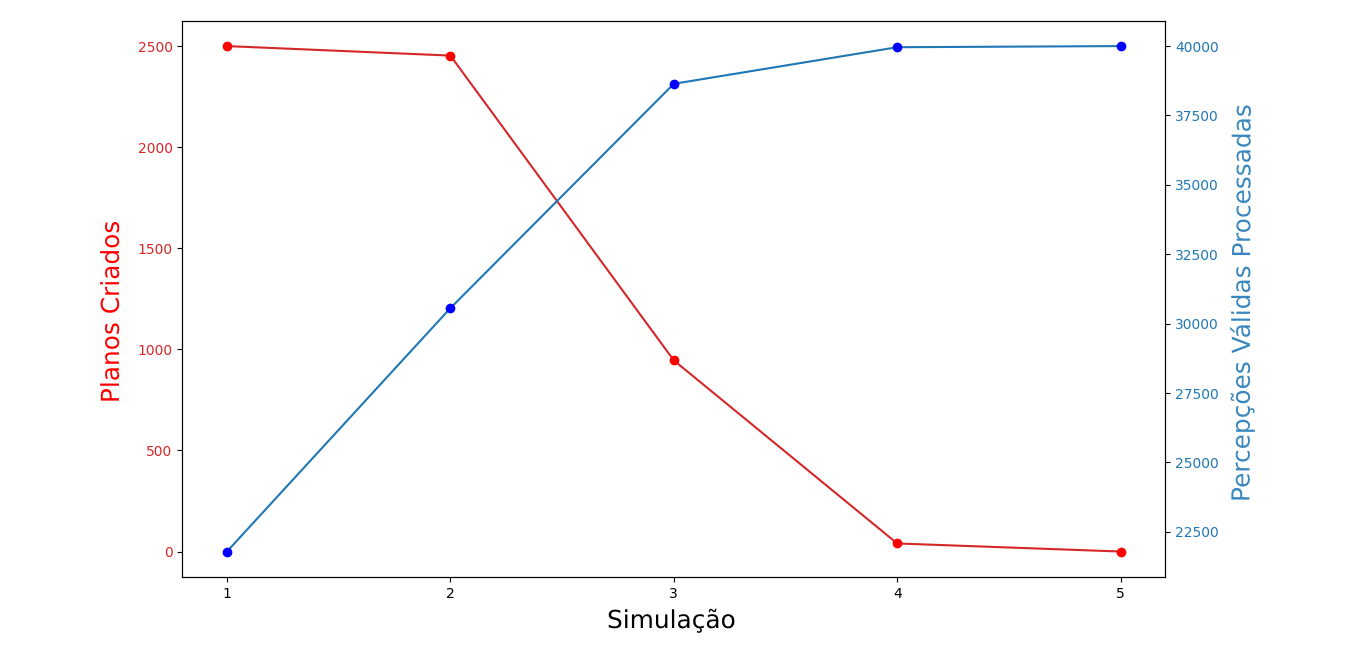
\includegraphics[width=\textwidth]{images/perceptions_vs_plans.png}
     \legend{Fonte: Autor.}
    \label{fig:perceptions_v_plans-experiment3}
\end{figure}

\section{Análise do modelo}

O principal objetivo dos experimentos era validar as ideias principais que compõem a proposta do modelo HAIL. Como as simulações foram realizadas sem ambiente e com um agente qualquer, os dados obtidos não podem ser usados como parâmetro de análise direta das qualidades do modelo, mas sim de seu funcionamento.

O primeiro experimento demonstrou que o módulo de ilusão e alucinação funciona como previsto: simulações com mais percepções inválidas e menor tempo médio de planejamento automatizado resultam em menos tempo virtual gasto e mais planos criados. Os grupos representados na Figura \ref{fig:pc_occurrences} demostram isso. As seis ocorrências do valor aproximado de 250 planos criados possuem PPI de 5\%. A única simulação com esse PPI que possui uma quantidade de planos criados aproximada aos valores das simulações com PPI 95\% possui TMA baixo e TMC e NPC altos, ou seja, muitos processos de planejamento automatizado são executados todos os ciclos, aumentando o número de planos criados. As demais simulações com esse PPI ou possuem poucas percepções por ciclo, ou o bloco avaliador não consegue enviar tantas anomalias para o planejamento automatizado devido aos valores de TMC e TMA.

Um dos objetivos do trabalho é criar um modelo capaz de aprender com as anomalias recebidas pelo agente através da percepção, e por isso o segundo e o terceiro experimentos abordam o mecanismo de aprendizado do HAIL. Com esses experimentos foi possível observar que o processo de seleção de anomalias que serão enviadas para o bloco de planejamento automatizado, desempenhado pelo bloco avaliador, é funcional.

O cenário ideal representado pelo experimento 3, onde todas as anomalias da primeira simulação se tornam parte do contexto do agente após poucas iterações, não tem como existir em uma situação real na qual a possibilidade de anomalias não é limitado por um gerador. Apesar disso, o experimento serve para demonstrar o funcionamento do módulo de ilusão e alucinação, pois os planos que são adicionados ao longo das simulações reduzem o tempo virtual e aumentam o número de percepções válidas processadas.

Com os resultados obtidos com os experimentos é possível afirmar que o modelo se comporta da maneira esperada, mas não é possível chegar a nenhuma conclusão relacionada à efetividade do modelo. Alguns cenários se mostraram favoráveis ao HAIL, como as simulações que possuem um grande volume de anomalias e baixo tempo de planejamento automatizado. Apesar disso, experimentos com cenários realistas e implementações acopladas a arquiteturas reais são necessários para validar que o modelo se comporta bem sob tais circunstâncias.